\documentclass{beamer}

\usepackage{xcolor}
\usepackage{tikz}
\usepackage{adjustbox}
\usepackage{booktabs}
\usepackage{tabularx}
\usepackage[center]{caption}

\usetikzlibrary{automata,positioning,shapes.multipart}

\usetheme{metropolis}           % Use metropolis theme

\setbeamerfont{bibliography item}{size=\tiny}
\setbeamerfont{bibliography entry author}{size=\tiny}
\setbeamerfont{bibliography entry title}{size=\tiny}
\setbeamerfont{bibliography entry location}{size=\tiny}
\setbeamerfont{bibliography entry note}{size=\tiny}


\newcommand{\Mimc}{\textnormal{MiMC}}
\newcommand{\Mimchash}{\textnormal{MiMCHash}}
\newcommand{\Hades}{\textnormal{\textsc{Hades}}}
\newcommand{\Poseidon}{\textnormal{\textsc{Poseidon}}}
\newcommand{\Rescue}{\textnormal{\textit{Rescue}}}
\newcommand{\Griffin}{\textnormal{\textsc{Griffin}}}
\newcommand{\Horst}{\textnormal{\texttt{Horst}}}
\newcommand{\Anemoi}{\textnormal{\texttt{Anemoi}}}
\newcommand{\Flystel}{\textnormal{\texttt{Flystel}}}
\newcommand{\Arion}{\textnormal{\textsf{Arion}}}
\newcommand{\Arionp}{\textnormal{\Arion-\(\pi \)}}
\newcommand{\Aarion}{\textnormal{\(\alpha \)-\Arion}}
\newcommand{\Arionhash}{\textnormal{\textsf{ArionHash}}}
\newcommand{\Aarionhash}{\textnormal{\(\alpha \)-\Arionhash}}

\title{Interview presentation}
\date{\today}
\author{Stefano Trevisani}
\institute{Università degli Studi di Udine \and Alpen Adria Universit\"{a}t Klagenfurt}

\begin{document}
\maketitle

\begin{frame}{ZK-SNARKs, what?}
  \emph{Zero-Knowledge Succinct Non-interactive ARgument of Knowledge}:
  \begin{itemize}
    \item A multidisciplinary topic: math, complexity, cryptography\footnote{
      A few milestones:~\cite{GoldwasserMR1989,Shamir1992,Damgard1993,Micali2000,GennaroGPR2012,Groth2016}.
    }. 
    \item \textcolor{teal}{Prover} wants to prove a statement, might be dishonest!
    \item \textcolor{orange}{Verifier} wants to verify the proof, might be curious!
    \item \textcolor{teal}{Prover} does not want to disclose secrets: \textbf{Zero-Knowledge}.
    \item \textcolor{orange}{Verifier} does not want to waste time: \textbf{Succinct} proof.
    \item \textcolor{teal}{Prover} proves once and for all: \textbf{Non-interactive}.
    \item Parties are ``not too powerful'': \textbf{ARgument of Knowledge}.
  \end{itemize}
\end{frame}

\begin{frame}{ZK-SNARKs, why?}
  Many useful applications! For example:
  \begin{itemize}
    \item Cloud computing~\cite{ParnoGHR2013}.
    \item Households figuring out their bills privately.
    \item \textbf{Anonymous transactions on the blockchain}~\cite{SassonCGGMTV2014}.
  \end{itemize}
\end{frame}

\begin{frame}{The Blockchain}
  \begin{figure}
    \centering
    \adjustbox{max height=128pt,keepaspectratio}{
    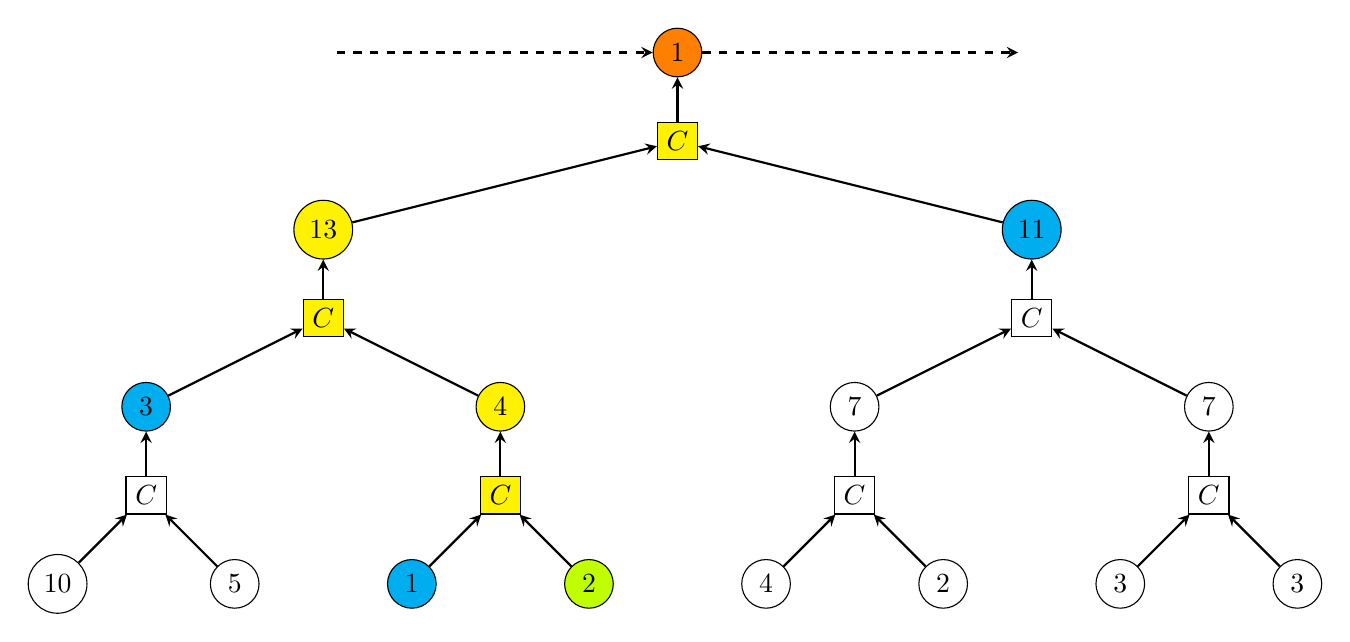
\begin{tikzpicture}[node distance={32pt}, node/.style = {draw, circle},on grid=true]
      \node[node] (y1) {\(10\)};
      \node[node,draw=none] (m1) [right of=y1] {};
      \node[node] (y2) [right of=m1] {\(5\)};
      \node[node,draw=none] (m2) [right of=y2] {};
      \node[node,fill=cyan] (y3) [right of=m2] {\(1\)};
      \node[node,draw=none] (m3) [right of=y3] {};
      \node[node,fill=lime] (y4) [right of=m3] {\(2\)};
      \node[node,draw=none] (m4) [right of=y4] {};
      \node[node] (y5) [right of=m4] {\(4\)};
      \node[node,draw=none] (m5) [right of=y5] {};
      \node[node] (y6) [right of=m5] {\(2\)};
      \node[node,draw=none] (m6) [right of=y6] {};
      \node[node] (y7) [right of=m6] {\(3\)};
      \node[node,draw=none] (m7) [right of=y7] {};
      \node[node] (y8) [right of=m7] {\(3\)};

      \node[node,shape=rectangle] (d1) [above of=m1] {\(C\)};
      \node[node,draw=none] (m8) [above of=m2] {};
      \node[node,shape=rectangle,fill=yellow] (d2) [above of=m3] {\(C\)};
      \node[node,draw=none] (m9) [above of=m4] {};
      \node[node,shape=rectangle] (d3) [above of=m5] {\(C\)};
      \node[node,draw=none] (m10) [above of=m6] {};
      \node[node,shape=rectangle] (d4) [above of=m7] {\(C\)};

      \node[node,fill=cyan] (x1) [above of=d1] {\(3\)};
      \node[node,draw=none] (n1) [above of=m8] {};
      \node[node,fill=yellow] (x2) [above of=d2] {\(4\)};
      \node[node,draw=none] (n2) [above of=m9] {};
      \node[node] (x3) [above of=d3] {\(7\)};
      \node[node,draw=none] (n3) [above of=m10] {};
      \node[node] (x4) [above of=d4] {\(7\)};
      \node[node,shape=rectangle,fill=yellow] (c1) [above of=n1] {\(C\)};
      \node[node,shape=rectangle] (c2) [above of=n3] {\(C\)};

      \node[node,fill=yellow] (x5) [above of=c1] {\(13\)};
      \node[node,draw=none] (n3) [above of=n2] {};
      \node[node,draw=none] (n4) [above of=n3] {};
      \node[node,fill=cyan] (x6) [above of=c2] {\(11\)};
      \node[node,shape=rectangle,fill=yellow] (c3) [above of=n4] {\(C\)};

      \node[node,fill=orange] (x7) [above of=c3] {\(1\)};
      \node[node,draw=none] (n5) [left =128pt of x7] {};
      \node[node,draw=none] (n6) [right =128pt of x7] {};


      \draw[-stealth,thick] (y1) to (d1);
      \draw[-stealth,thick] (y2) to (d1);
      \draw[-stealth,thick] (y3) to (d2);
      \draw[-stealth,thick] (y4) to (d2);
      \draw[-stealth,thick] (y5) to (d3);
      \draw[-stealth,thick] (y6) to (d3);
      \draw[-stealth,thick] (y7) to (d4);
      \draw[-stealth,thick] (y8) to (d4);

      \draw[-stealth,thick] (d1) to (x1);
      \draw[-stealth,thick] (d2) to (x2);
      \draw[-stealth,thick] (d3) to (x3);
      \draw[-stealth,thick] (d4) to (x4);


      \draw[-stealth,thick] (x1) to (c1);
      \draw[-stealth,thick] (x2) to (c1);
      \draw[-stealth,thick] (x3) to (c2);
      \draw[-stealth,thick] (x4) to (c2);

      \draw[-stealth,thick] (c1) to (x5);
      \draw[-stealth,thick] (c2) to (x6);

      \draw[-stealth,thick] (x5) to (c3);
      \draw[-stealth,thick] (x6) to (c3);

      \draw[-stealth,thick] (c3) to (x7);

      \draw[dashed,-stealth,thick] (n5) to (x7);
      \draw[dashed,-stealth,thick] (x7) to (n6);
    \end{tikzpicture}
    }
  \end{figure}
  \begin{itemize}
    \item Groups of transactions are leaves of a \emph{Merkle tree}~\cite{Merkle1988}.
    \item Bottom-up computation using a \textbf{compression function}.
    \item The root contains the \emph{commitment} (among other data).
    \item Verify a commitment following the \emph{authentication path}.
  \end{itemize}
\end{frame}

\begin{frame}{Compression functions}
  One-way compression functions (OWCF):
  \begin{itemize}
    \item Many (e.g.\  \(2\)) inputs and few (e.g.\  \(1\)) outputs.
    \item Easy to compute, but hard to invert (and find collisions).
    \item Usually derived from one-way permutations.
    \item Standard designs (SHA~\cite{Dang2015}) work over \emph{boolean fields}.
    \item Davies-Meyer~\cite{Preneel2005}, sponge~\cite{BertoniDPA2007}\dots
  \end{itemize}
  \begin{figure}
    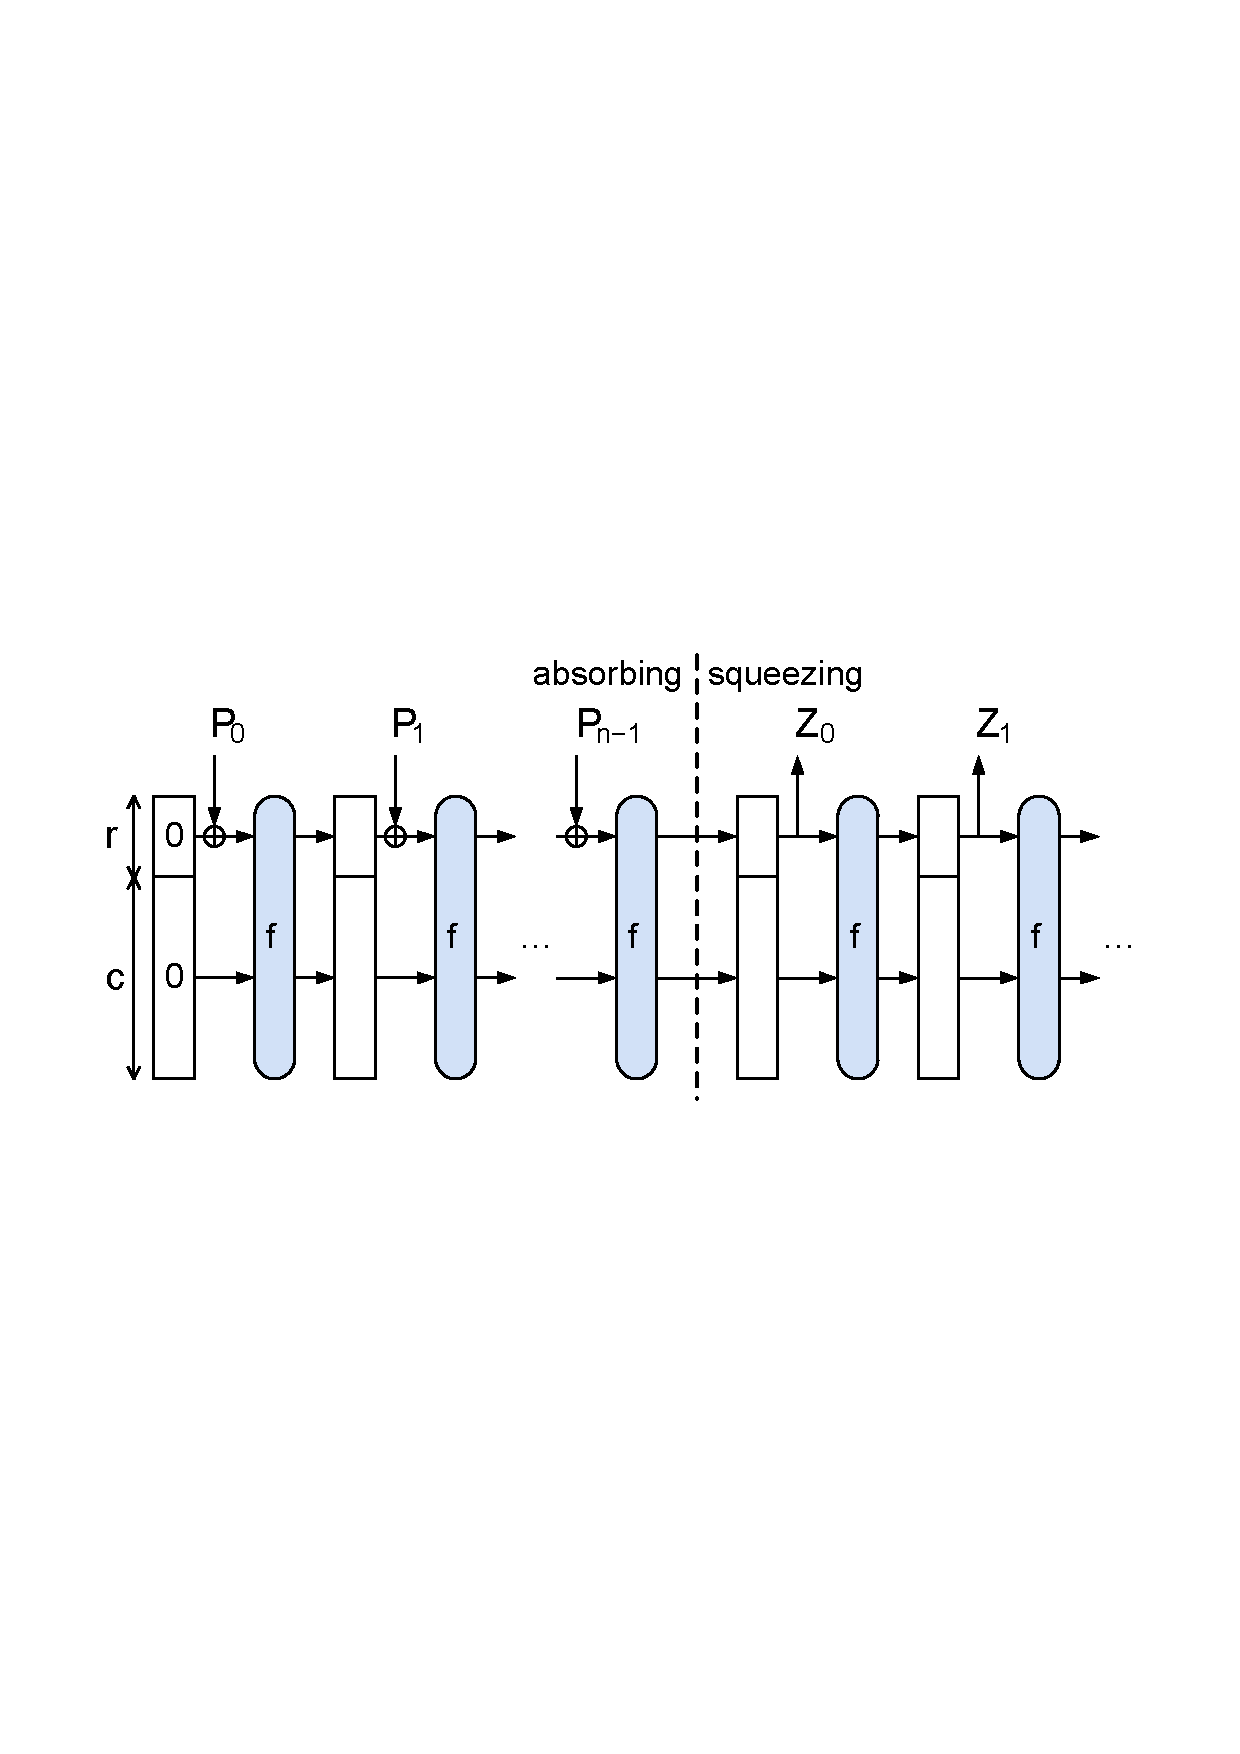
\includegraphics[scale=0.4]{SpongeConstruction.pdf}
  \end{figure}
\end{frame}

\begin{frame}{ZK-SNARK and compression functions}
  SHA is very fast natively, but what about in ZK-SNARK\@?
  \begin{itemize}
    \item Efficient ZK-SNARKs over prime fields \(\mathbb{F}_p\)~\cite{GennaroGPR2012}.
    \item Input-output relationship as bi-linear constraints (R1CS)~\cite{SassonCTV2013}.
    \item One multiplication \(=\) one constraint. 
    \item What about SHA-256? 25000\texttt{+} constraints!
    \item Can we do better?
  \end{itemize}  
\end{frame}

\begin{frame}{\Mimc}
  Minimal Multiplicative Complexity (\Mimc) hash function~\cite{AlbrechtGRRT2016}:
  \begin{itemize}
    \item Extremely simple: \emph{round function} is \(x^3 + c\)\footnote{Warning: might not be a 
          permutation!}.
    \item Many rounds to be secure against \emph{algebraic attacks}.
    \item \Mimchash-256: 640 constraints.
    \item Can we do better?
  \end{itemize}  
\end{frame}

\begin{frame}{\Poseidon}
  Many improvements in the last years, \Poseidon~\cite{GrassiKRRS2021}\footnote{
    See also:~\cite{GrassiHRSWW2022,BouvierBCPSVW2022,AlyABDS2019}.}:
  \begin{itemize}
    \item Partial \emph{substitution-permutation network} (SPN) rounds.
    \item Full SPN for classic attacks (linear, differential\dots).
    \item Partial SPN for algebraic attacks (interpolation, Gr\"{o}bner\dots).
    \item \Poseidon-256: 276 constraints.
    \item Can we do better?
  \end{itemize}
\end{frame}

\begin{frame}{\Arion}
  Our design \Arion~\cite{RoyST2023}:
  \begin{itemize}
    \item Builds on the GTDS algebraic framework~\cite{RoyS2022}.
    \item Two variants: \Arion{} and \Aarion.
    \item \Aarionhash-256: 76 constraints.
  \end{itemize}
\end{frame}

\begin{frame}{Comparisons}
  \texttt{libsnark}: used by ZCash~\cite{SassonCGGMTV2014} for its blockchain.\\
  We used it to implement:
  \begin{itemize}
    \item Several primitives designed for ZK-SNARK, including ours.
    \item A self-parametrizing Merkle tree.
    \item A new mode of hash, the Augmented Binary tRee~\cite{AndreevaBR2021}.
  \end{itemize}
  \begin{table}
    \caption*{Proof generation times for MT commitments over 256-bit prime fields}
    \centering
        \begin{tabular}{c c c c}  
          \toprule
          Tree height & \Aarionhash{} & \Griffin{} & \Poseidon{} \\
          \midrule
          \(4\)   & \(73\) ms  & \(88\) ms & \(186\) ms  \\
          \(8\)   & \(145\) ms & \(181\) ms & \(386\) ms  \\
          \(16\)  & \(278\) ms & \(338\) ms & \(745\) ms  \\
          \(32\)  & \(509\) ms & \(622\) ms & \(1422\) ms \\
          \bottomrule
        \end{tabular}
  \end{table}
\end{frame}


\begin{frame}
  \begin{center}
    \rule{\textwidth}{0.5pt}
    \huge{\(\mathcal{T}\mathit{he}\)} \ \huge{\(\mathcal{E}\mathit{nd}\)}\\
    \Large{\emph{Thank you for your attention!}}
    \rule{\textwidth}{0.5pt}
  \end{center}
\end{frame}

\begin{frame}[allowframebreaks]  
  \bibliographystyle{alpha}
  \bibliography{biblio.bib}
\end{frame}

\end{document}
